\documentclass[11pt,a4paper]{article}

% ------------------------------------------------
% PAQUETES
% ------------------------------------------------
\usepackage[utf8]{inputenc}
\usepackage[T1]{fontenc}
\usepackage[spanish,provide=*]{babel}
\usepackage{lmodern}
\usepackage{listings}

\lstset{
    language=C,
    basicstyle=\ttfamily\small,
    frame=single,
    breaklines=true,
    columns=fullflexible,
    keepspaces=true
}

\usepackage{geometry}
\geometry{
    top=2.2cm,
    bottom=2.2cm,
    left=2.5cm,
    right=2.5cm
}

\usepackage{amsmath}
\usepackage{amssymb}
\usepackage{graphicx}
\usepackage{booktabs}
\usepackage{array}
\usepackage{tabularx}
\usepackage{float}
\usepackage{xcolor}
\usepackage{enumitem}
\usepackage{xurl}
\usepackage{hyperref}

\hypersetup{
    colorlinks=true,
    linkcolor=black,
    urlcolor=blue,
    citecolor=black
}

\setlength{\parindent}{0pt}
\setlength{\parskip}{0.7em}

% ------------------------------------------------
% DOCUMENTO
% ------------------------------------------------
\begin{document}

\begin{center}
    {\LARGE \textbf{Pruebas de entrada: Aviónica}}\\[0.4cm]
    {\large Faraday Rocketry UPV}\\[0.8cm]
    {\Large \textbf{Ejercicio 1: Selección de microcontrolador y configuración básica}}
\end{center}

\vspace{0.5cm}

\hrule
\vspace{0.5cm}

% ================================================================
\section*{Enunciado}
% ================================================================

En el departamento de aviónica se trabaja principalmente con
microcontroladores del ecosistema STM32.

\begin{enumerate}[label=\alph*.]

    \item Seleccionar un microcontrolador STM32 para la aviónica de vuelo
    y justificar la elección atendiendo a aspectos como memoria,
    potencia de cálculo, consumo y periféricos.

    \item Configurar un proyecto básico en STM32CubeMX que cuente con:
    \begin{itemize}
        \item Al menos un bus SPI\@.
        \item Al menos un bus I\textsuperscript{2}C.
        \item La configuración necesaria para utilizar un programador
        ST-LINK\@.
    \end{itemize}

\end{enumerate}

% ================================================================
\section{Selección del microcontrolador}
% ================================================================

El microcontrolador constituye el núcleo de procesamiento de la aviónica de vuelo. Entre sus funciones se encuentran la adquisición de datos procedentes de los sensores, su procesamiento, el almacenamiento de información y la comunicación con el resto de subsistemas.

Para realizar la selección se estudiarán principalmente los siguientes criterios:
\begin{itemize}

    \item Arquitectura y potencia de cálculo.
    \item Memoria Flash y memoria RAM\@.
    \item Periféricos de comunicación disponibles.
    \item Número de entradas y salidas.
    \item Consumo energético.
    \item Margen para incluir otras funciones no contempladas inicialmente en nuestro sistema.

\end{itemize}

% ================================================================
\subsection{Arquitectura propuesta y requisitos de conectividad}
% ================================================================

Como hipótesis de partida, se considera una arquitectura formada por:

\begin{itemize}

    \item un receptor GNSS conectado mediante UART\@;

    \item una IMU y una memoria externa compartiendo un mismo bus SPI\@;

    \item un barómetro conectado mediante I\textsuperscript{2}C\@;

    \item una interfaz de programación y depuración mediante ST-LINK/SWD\@.

\end{itemize}

Además, el sistema deberá permitir posteriormente la incorporación de un
transceptor de radio para telemetría. Al no haberse seleccionado todavía
dicho dispositivo, su interfaz concreta no se fija en esta fase. No
obstante, se deberá conservar margen suficiente de periféricos y GPIO
para su integración.

La arquitectura propuesta permite estimar unos requisitos mínimos de
conectividad para la selección inicial del microcontrolador.

\begin{table}[H]

    \centering
    \renewcommand{\arraystretch}{1.3}

    \begin{tabularx}{\textwidth}{
        >{\raggedright\arraybackslash}p{3.2cm}
        >{\centering\arraybackslash}p{2.7cm}
        >{\raggedright\arraybackslash}X
    }

        \toprule
        \textbf{Función} &
        \textbf{Conexiones} &
        \textbf{Especificación} \\
        \midrule

        SPI compartido &
        \textbf{5 pines} &
        SCK, MOSI y MISO compartidos, junto con una señal
        \textit{Chip Select} independiente para la IMU y la memoria. \\

        I\textsuperscript{2}C &
        \textbf{2 pines} &
        SCL y SDA\@. Ambas líneas requerirán resistencias
        \textit{pull-up} en la placa. \\

        UART &
        \textbf{2 pines} &
        TX y RX para la comunicación bidireccional con el receptor GNSS\@. \\

        SWD &
        \textbf{2 pines} &
        SWDIO y SWCLK para programación y depuración mediante ST-LINK\@. \\

        Reinicio &
        \textbf{NRST} &
        Pin dedicado de reinicio. Resulta conveniente llevarlo al
        conector de programación y depuración. \\

        Referencia eléctrica &
        \textbf{GND y VTref} &
        Masa y referencia de tensión del circuito objetivo necesarias
        para el programador, según el modelo de ST-LINK empleado. \\

        \bottomrule

    \end{tabularx}

    \caption{Requisitos mínimos de conectividad considerados para la selección del microcontrolador.}

\end{table}

La arquitectura definida requiere, por tanto, once señales asociadas a
interfaces digitales: cinco para SPI, dos para I\textsuperscript{2}C,
dos para UART y dos para SWD, además del pin dedicado NRST\@.

Este número no debe interpretarse simplemente como once GPIO libres,
ya que los pines seleccionados deben ser compatibles simultáneamente con
las funciones alternativas correspondientes.

Además, se deberá conservar margen para la futura interfaz de radio y
para posibles señales adicionales de interrupción, habilitación o
control de los periféricos.

\newpage
% ================================================================
\subsection{Tareas del microcontrolador}
% ================================================================

A partir de la arquitectura planteada, las principales tareas que deberá
realizar el microcontrolador durante el vuelo son:

\begin{table}[H]

\centering
\small
\renewcommand{\arraystretch}{1.3}

\begin{tabularx}{\textwidth}{
    >{\bfseries\raggedright\arraybackslash}p{3.0cm}
    >{\raggedright\arraybackslash}X
    >{\raggedright\arraybackslash}X
}

\toprule
Tarea & Qué resuelve & Ejemplo \\
\midrule

Lectura de sensores &
Obtener periódicamente las medidas de los periféricos. &
Leer presión, aceleración, velocidad angular o posición. \\

Calibración &
Corregir offset, escala u otros errores conocidos de los sensores. &
Eliminar un error de cero antes de utilizar una medida. \\

Filtrado &
Reducir ruido y variaciones de las medidas que no representan cambios
relevantes del vuelo. &
Suavizar la medida de presión para obtener una estimación de altura más estable. \\

Identificación de fases &
Interpretar la evolución de las medidas para determinar el estado del vehículo. &
Distinguir entre espera, ascenso y descenso. \\

Registro &
Guardar las medidas y estados para analizarlos posteriormente. &
Almacenar periódicamente los datos de vuelo en memoria externa. \\

Telemetría &
Preparar los datos necesarios para transmitir información hacia tierra. &
Construir paquetes con las principales variables de vuelo para su posterior
transmisión mediante el transceptor de radio. \\

\bottomrule

\end{tabularx}

\caption{Tareas principales del microcontrolador durante el vuelo}%
\label{tab:tareas_microcontrolador}

\end{table}

% ================================================================
\subsection{Criterios de evaluación de los candidatos}
% ================================================================

Una vez comprobada la compatibilidad básica de interfaces, los
microcontroladores candidatos se compararán mediante los siguientes
criterios:

\begin{table}[H]

\centering
\renewcommand{\arraystretch}{1.3}

\begin{tabularx}{\textwidth}{
    >{\bfseries\raggedright\arraybackslash}p{4cm}
    >{\raggedright\arraybackslash}X
}

\toprule
Criterio & Qué se evaluará \\
\midrule

Capacidad de cálculo &
Capacidad del microcontrolador para ejecutar adquisición, procesamiento,
filtrado, registro y gestión del sistema dentro de los tiempos requeridos.
La validación definitiva deberá realizarse posteriormente sobre la
implementación real. \\

RAM &
Espacio disponible para buffers, variables y memoria de trabajo,
manteniendo un margen para ampliaciones. \\

Flash interna &
Espacio disponible para el programa, bibliotecas y constantes,
manteniendo igualmente un margen suficiente. \\



DMA &
Disponibilidad de transferencia directa de memoria que permita reducir
la intervención de la CPU en operaciones repetitivas de comunicación o
adquisición. \\

FPU &
Presencia de una unidad de coma flotante que pueda acelerar determinadas
operaciones numéricas realizadas sobre datos de sensores. \\

Consumo &
Consumo en funcionamiento y en los modos de bajo consumo que puedan
resultar relevantes, comparando los dispositivos bajo condiciones
equivalentes. \\

Margen de expansión &
Disponibilidad de periféricos, memoria y GPIO adicionales para integrar
posteriormente otros sensores o el sistema de radio. \\

Coste &
Precio unitario aproximado del microcontrolador. \\
\bottomrule

\end{tabularx}

\caption{Criterios utilizados para comparar los microcontroladores candidatos}%
\label{tab:criterios_microcontrolador}

\end{table}

% ================================================================
\subsection{Comparación de alternativas}
% ================================================================

Como primera comparación se consideran tres microcontroladores STM32 con
características diferentes de memoria, arquitectura y frecuencia máxima
de funcionamiento:

\begin{table}[H]

\centering
\footnotesize
\renewcommand{\arraystretch}{1.3}

\begin{tabularx}{\textwidth}{
    >{\bfseries\raggedright\arraybackslash}X
    >{\centering\arraybackslash}p{3.0cm}
    >{\centering\arraybackslash}p{3.0cm}
    >{\centering\arraybackslash}p{3.0cm}
}

\toprule
Criterio &
STM32G071RBT6 &
STM32F401RET6 &
STM32L476RGT6 \\
\midrule

Núcleo &
Cortex-M0+ &
Cortex-M4 &
Cortex-M4 \\

Frecuencia máxima &
64 MHz &
84 MHz &
80 MHz \\

FPU &
No &
Sí &
Sí \\

Flash &
128 KB &
512 KB &
1024 KB \\

RAM &
36 KB &
96 KB &
128 KB \\

Precio unitario orientativo &
$\sim$4,3923\,€ &
$\sim$
7,7319\,€ &
$\sim$10,55\,€ \\
\bottomrule

\end{tabularx}

\caption{Comparación inicial de los microcontroladores considerados.
Datos obtenidos de las fichas de STMicroelectronics~\cite{st_g071,st_f401,st_l476}.
Los precios se consultaron en Farnell el 24 de septiembre de 2026~\cite{farnell}.}

\end{table}

Cada STM32 contemplado responde a un perfil de uC diferente. El primero responde a una configuración más básica, sin FPU y con menos frecuencia máxima y memoria que los otros dos contemplados. El segundo es un uC centrado en el rendimiento, siendo éste el que tiene una mayor frecuencia máxima, pero con menor memoria que el último, que se trata de un uC de bajo consumo.

La FPU puede acelerar parte de los cálculos en coma flotante, aunque no implica que el cálculo de logaritmos se realice íntegramente por hardware, al ser funciones de biblioteca. Aún así, a priori, la presencia de FPU si bien no tendría por qué ser un criterio determinante, sí lo consideraremos como una ventaja para los dos últimos modelos seleccionados. Las comunicaciones periódicas con los periféricos también podrían beneficiarse del DMA, al reducir la intervención de la CPU durante determinadas transferencias. Los tres candidatos disponen de DMA, si bien su uso concreto deberá configurarse y justificarse en la implementación.

\subsubsection{Estimación de la memoria}

Para estimar cuánta memoria Flash y RAM necesitará el programa,
realizaremos una implementación básica de algunas de las funciones
previstas: filtrado de medidas, cálculo de altura e identificación de
fases de vuelo. Una vez compilada, compararemos la ocupación del
programa y de sus variables y buffers con la memoria disponible en
cada candidato. Esta estimación será parcial, pues aún no incluirá
todos los controladores y funciones del sistema final.

Para realizar esta estimación inicial se ha escogido el
STM32L476RGT6 como microcontrolador de ejemplo. En esta fase no se
pretende comparar mediciones exactas entre los tres candidatos, sino
obtener una referencia del orden de magnitud de la memoria Flash y
RAM necesarias. La ocupación concreta puede variar entre
microcontroladores por las diferencias en sus arquitecturas,
bibliotecas y configuraciones de compilación.

Para construir el programa de prueba se utilizó la asignación de interfaces
y pines descrita para el STM32L476RGT6. La configuración se recoge en la
Tabla~\ref{tab:asignacion_pines}.

%
Ejecutando el programa correspondiente a la inicialización básica del
microcontrolador y de los periféricos configurados, obtenemos una ocupación
de 13\,864 bytes de memoria Flash y 1\,904 bytes de RAM\@. En el
STM32L476RGT6, los 128 KB de RAM se distribuyen en 96 KB de RAM principal
y 32 KB de RAM2; esta última región no se utiliza en la compilación actual.
Estas cifras corresponden únicamente a la inicialización de los periféricos.
Las funciones añadidas después y la integración realizada en el ejercicio 2
se comparan en la Tabla~\ref{tab:ocupacion_flash_prueba}.

\paragraph{Implementación de funciones representativas.}

Para observar cómo aumenta la ocupación de memoria al incorporar funciones
de la aplicación, se añadieron progresivamente las funciones deseadas: un filtro de altura, una
conversión de presión a altura relativa o los estados lógicos que representan los estados del vuelo. Todo esto empleando entradas ficticias
variables. Las funciones y el código utilizado para ejecutarlas se muestran
en el anexo~\ref{anexo:estimacion_flash}.

El filtrado se implementó mediante la relación
\begin{equation}
    h_{\mathrm{filtrada},i}
    =h_{\mathrm{filtrada},i-1}
    +\alpha\left(h_{\mathrm{baro},i}
    -h_{\mathrm{filtrada},i-1}\right),
\end{equation}
donde se utilizó $\alpha=0{,}25$ únicamente como valor de prueba.

Para convertir la presión en altura relativa se utilizó, como aproximación,
un modelo de atmósfera isoterma:
\begin{equation}
    h \simeq \frac{RT}{g}
    \ln\left(\frac{p_0}{p}\right),
\end{equation}
donde $p_0$ representa la presión en el punto de lanzamiento, $p$ la
presión actual y $T$ la temperatura supuesta constante. En el programa
de prueba se emplearon $T=288{,}15\ \mathrm{K}$ y un valor ficticio
$p_0=101\,325\ \mathrm{Pa}$. En una implementación con barómetro, $p_0$
se obtendría mediante una medida previa al lanzamiento.

Para estudiar la identificación del descenso, se incorporó un
historial circular de 20 alturas filtradas. Este permite comparar
la altura actual con la obtenida aproximadamente 0,2 segundos antes (hemos usado una frecuencia de 100Hz para el ejemplo).
El prototipo conserva además la máxima altura estimada y declara
descenso cuando se cumplen dos condiciones: una caída de al menos
2 m respecto a ese máximo y una disminución de al menos 1 m en la
ventana de 0,2 segundos. La condición debe cumplirse en 50
comprobaciones; se toleran hasta dos resultados desfavorables
consecutivos antes de reiniciar el contador. Los umbrales anteriores son valores de prueba. La generación de medidas simuladas y la lógica utilizada para
detectar el descenso se muestran en el
Anexo~\ref{anexo:simulacion_descenso}.

\begin{table}[H]
    \centering
    \renewcommand{\arraystretch}{1.2}
    \begin{tabular}{p{7.5cm}rrr}
        \toprule
        Versión compilada & Flash & RAM principal & RAM2 \\
        \midrule
        Inicialización de periféricos
            & 13\,864 B & 1\,904 B & 0 B \\
        Inicialización y filtro
            & 14\,080 B & 1\,920 B & 0 B \\
        Inicialización, filtro y conversión de presión
            & 14\,920 B & 2\,312 B & 0 B \\
        Más simulación de ascenso y descenso
            & 15\,040 B & 2\,312 B & 0 B \\
        Más historial de 20 alturas
            & 15\,160 B & 2\,400 B & 0 B \\
        Más identificación del descenso
            & 15\,344 B & 2\,408 B & 0 B \\
        Ejercicio 2: integración de sensores y recepción GNSS
            & 27\,048 B & 2\,736 B & 0 B \\
        \bottomrule
    \end{tabular}
    \caption{Ocupación de las versiones de prueba del ejercicio 1 y de la
    ampliación del ejercicio 2, compiladas para el STM32L476RGT6. La RAM principal
    corresponde a una región de 96 KB\@; los 32 KB de RAM2 se muestran
    por separado.}%
    \label{tab:ocupacion_flash_prueba}
\end{table}

En el ejercicio 2 se amplía el programa provisional del ejercicio 1. Se
incorporan la identificación y lectura de dos barómetros LPS22DF, la
combinación de sus muestras para calcular la altura, la adquisición del
acelerómetro de bajo rango y del giróscopo de la LSM6DSV320X, la
configuración de su canal de alto rango y la recepción de bytes del GNSS.
El canal de alto rango todavía no se lee y los bytes GNSS no se interpretan.
En esa compilación, la ocupación aumenta en 11\,704 B de Flash y 328 B de RAM
respecto a la última versión del ejercicio 1. Las cifras proceden de los
archivos ejecutables compilados para el STM32L476RGT6; no incluyen la memoria
externa ni demuestran el funcionamiento con sensores físicos.
La memoria disponible en el STM32L476RGT6 presenta margen respecto a esta
implementación. El tamaño obtenido para este microcontrolador no permite
afirmar que el mismo código ocupe idéntica memoria en los otros candidatos.

\begin{table}[H]
    \centering
    \renewcommand{\arraystretch}{1.2}
    \begin{tabular}{lrrrr}
        \toprule
        Microcontrolador
        & Flash disponible & Flash ocupada
        & RAM disponible & RAM ocupada \\
        \midrule
        STM32G071RBT6 & 128 KB   & 20,64\,\% & 36 KB  & 7,42\,\% \\
        STM32F401RET6 & 512 KB   &  5,16\,\% & 96 KB  & 2,78\,\% \\
        STM32L476RGT6 & 1\,024 KB &  2,58\,\% & 128 KB & 2,09\,\% \\
        \bottomrule
    \end{tabular}
    \caption{Porcentaje que representarían los 27\,048 B de Flash y
    2\,736 B de RAM de la ampliación del ejercicio 2 respecto a la capacidad
    nominal de cada candidato. Se trata de una comparación ilustrativa:
    el programa solo se ha compilado para el STM32L476RGT6.}%
    \label{tab:comparacion_memoria_candidatos}
\end{table}

\subsubsection{Capacidad de cálculo y consumo}

La selección del microcontrolador también debe considerar si puede
completar a tiempo las operaciones necesarias durante el vuelo. En nuestro ejemplo, antes de la
siguiente medida deberán haberse completado su adquisición, el
cálculo y filtrado de la altura y la actualización de la detección
de descenso. Por tanto, establecemos el siguiente requisito temporal
inicial:

\begin{equation}
t_{\text{adquisición}}
+t_{\mathrm{altura}}
+t_{\mathrm{filtrado}}
+t_{\text{detección}}
+t_{\mathrm{margen}}
\leq 10\,\mathrm{ms},
\label{eq:presupuesto_temporal}
\end{equation}

donde $t_{\mathrm{margen}}$ reserva tiempo para interrupciones y
variaciones en la duración de las operaciones. El registro y la
transmisión de datos podrían atenderse posteriormente mediante
buffers, siempre que no retrasen las tareas anteriores y que los
datos pendientes no se acumulen. Los tiempos de la
ecuación todavía no se han medido en el microcontrolador; por ello,
este requisito permite orientar la comparación, pero no demuestra
que alguno de los candidatos lo cumpla.

Analizaremos la capacidad de cálculo junto con el consumo
energético, ya que la energía consumida depende
tanto de la potencia como del tiempo de funcionamiento. Compararemos por ello las
especificaciones de consumo indicando las condiciones de medida,
sin deducir el consumo durante el vuelo únicamente a partir de
la frecuencia máxima de cada candidato.
\paragraph{Comparación inicial del consumo en modo activo}

Como primera referencia, se consultó en las hojas de datos de
STMicroelectronics la corriente típica de los tres candidatos
mientras ejecutan código desde la memoria Flash. La
Tabla~\ref{tab:consumo_run_candidatos} recoge un punto de
funcionamiento próximo a la frecuencia máxima de cada dispositivo.

\begin{table}[H]
    \centering
    \renewcommand{\arraystretch}{1.25}
    \begin{tabular}{p{3.6cm}ccp{6.2cm}}
        \toprule
        Microcontrolador
        & Frecuencia
        & Corriente típica
        & Condiciones indicadas en la hoja de datos \\
        \midrule
        STM32G071RBT6
        & 64 MHz
        & 6,4 mA
        & Código de prueba desde Flash; periféricos desactivados. \\

        STM32F401RET6
        & 84 MHz
        & 12,5 mA
        & Procesamiento desde Flash; periféricos desactivados. \\

        STM32L476RGT6
        & 80 MHz
        & 10,2 mA
        & Procesamiento desde Flash; periféricos desactivados y
          regulador interno. \\
        \bottomrule
    \end{tabular}
   \caption{Corrientes de referencia publicadas para los tres
microcontroladores bajo las condiciones indicadas en sus respectivas
fichas técnicas~\cite{st_g071,st_f401,st_l476}.}%
    \label{tab:consumo_run_candidatos}
\end{table}

En los puntos de funcionamiento consultados, el STM32G071RBT6
presenta la menor corriente típica. Sin embargo, estos valores
se han obtenido a distintas frecuencias y con programas de
ensayo diferentes. Tampoco incluyen el funcionamiento de los
periféricos previstos en nuestra aviónica. Por ello, la tabla
no permite determinar por sí sola qué microcontrolador
consumiría menos energía al realizar nuestras tareas.

En particular, el G071 carece de FPU, mientras que el F401 y
el L476 disponen de ella. Esto puede influir en el tiempo
necesario para efectuar los cálculos en coma flotante, pero
todavía no se ha medido el tiempo de ejecución del programa
en ninguno de los tres dispositivos.


Para obtener una primera referencia de energía consumida, se supone
que los tres microcontroladores trabajan durante un vuelo de
\(120\,\mathrm{s}\), alimentados a \(3{,}3\,\mathrm{V}\). Se considera que
permanecen el \(100\%\) de ese tiempo en modo \textit{Run}. Esta
hipótesis permite comparar las corrientes recogidas en los datasheets
sin estimar todavía cuánto tiempo dedicaría cada candidato al
procesamiento y cuánto podría permanecer en reposo.

En general, si el microcontrolador alternase entre ambos modos, la
energía consumida sería

\begin{equation}
E = V\left(
I_{\mathrm{Run}}\,t_{\mathrm{Run}}
+
I_{\mathrm{reposo}}\,t_{\mathrm{reposo}}
\right).
\end{equation}

Bajo la hipótesis adoptada,
\(t_{\mathrm{Run}}=120\,\mathrm{s}\) y
\(t_{\mathrm{reposo}}=0\), por lo que la expresión se reduce a

\begin{equation}
E_{\mathrm{ref}} =
V\,I_{\mathrm{Run,ref}}\,(120\,\mathrm{s}).
\end{equation}

Las corrientes utilizadas son valores de referencia obtenidos en
condiciones de ensayo de los fabricantes, con los periféricos
deshabilitados. Cabe esperar un consumo superior al habilitar y
utilizar los periféricos necesarios durante el vuelo. Además, la
corriente publicada para el STM32G071 corresponde a la ejecución de
un código reducido, diferente del procesamiento previsto en nuestra
aplicación. Por ello, \(E_{\mathrm{ref}}\) representa únicamente
el escenario definido por estas hipótesis, no una predicción del
consumo real en vuelo.

Bajo la hipótesis de funcionamiento continuo en modo \textit{Run},
la energía de referencia consumida durante los \(120\,\mathrm{s}\)
se calcula mediante

\begin{equation}
E_{\mathrm{ref}}
= V I_{\mathrm{Run,ref}}t,
\qquad
V=3{,}3\,\mathrm{V},
\quad t=120\,\mathrm{s}.
\end{equation}

\begin{table}[H]
    \centering
    \begin{tabular}{lrr}
        \toprule
        Microcontrolador & Corriente de referencia & Energía de referencia \\
        \midrule
        STM32G071RBT6 & 6,4 mA  & 2,53 J \\
        STM32F401RET6 & 12,5 mA & 4,95 J \\
        STM32L476RGT6 & 10,2 mA & 4,04 J \\
        \bottomrule
    \end{tabular}
    \caption{Energía calculada para \(120\,\mathrm{s}\) continuos en
    modo \textit{Run} y una alimentación supuesta de \(3{,}3\,\mathrm{V}\).
    Los resultados corresponden al escenario de referencia definido,
    no a una medición del consumo durante el vuelo.}%
    \label{tab:energia_referencia_uc}
\end{table}

La comparación anterior supone que los tres microcontroladores
permanecen continuamente en modo \textit{Run}. En una implementación
que permita entrar en un modo de bajo consumo entre muestras, los
candidatos que completen antes el procesamiento podrían disponer
de más tiempo de reposo. Por ello, una corriente mayor en modo
\textit{Run} no implica necesariamente una mayor energía consumida
por muestra o durante el vuelo.

La comparación de los modelos STM32F401, STM32L476 y STM32G071 todavía
no permite establecer cuál
consumiría menos energía en la aplicación real. Para ello sería necesario
conocer el tiempo de ejecución, la corriente en reposo y el coste de entrar
y salir de dicho modo. El F401 y el L476 podrían completar antes una tarea
y aprovechar más tiempo de reposo, pero su menor energía total aún no se ha
demostrado.
\subsubsection{Periféricos y asignación de pines}

Se ha comprobado que los tres candidatos permiten utilizar
simultáneamente las interfaces previstas, sin conflictos en la
asignación de pines: SPI1 en PA5, PA6 y PA7; dos señales CS
independientes en PA4 y PC4; I\textsuperscript{2}C1 en PB6 y PB7;
USART1 en PA9 y PA10; y SWD en PA13 y PA14. El pin de reinicio
se denomina NRST en los STM32F401RET6 y STM32L476RGT6, y
PF2-NRST en el STM32G071RBT6.

Por tanto, ninguno de los tres candidatos queda descartado por
los periféricos o pines necesarios para la arquitectura considerada.
Esta comprobación no incluye todavía las conexiones de una radio
ni de posibles actuadores futuros, por lo que se valora conservar
margen de pines para su incorporación.

La coexistencia de las interfaces previstas se comprobó inicialmente en
STM32CubeMX con el modelo STM32L476RGT6\@. Los pines
asignados se recogen en la Tabla~\ref{tab:asignacion_pines}. El resultado
en la herramienta se muestra en la Figura~\ref{fig:stm32_pinout}.

\begin{table}[H]
\centering
\renewcommand{\arraystretch}{1.3}

\begin{tabularx}{\textwidth}{
    >{\bfseries\raggedright\arraybackslash}p{5cm}
    >{\raggedright\arraybackslash}X
}

\toprule
Función & Pines \\
\midrule

SPI1 &
PA5, PA6, PA7 \\

CS de IMU y memoria &
PA4, PC4 \\

I\textsuperscript{2}C1 &
PB6, PB7 \\

USART1 para GNSS &
PA9, PA10 \\

SWD &
PA13, PA14 \\

\bottomrule
\end{tabularx}

\caption{Asignación de pines utilizada en la configuración del microcontrolador.}%
\label{tab:asignacion_pines}


\end{table}

\begin{figure}[H]
    \centering
    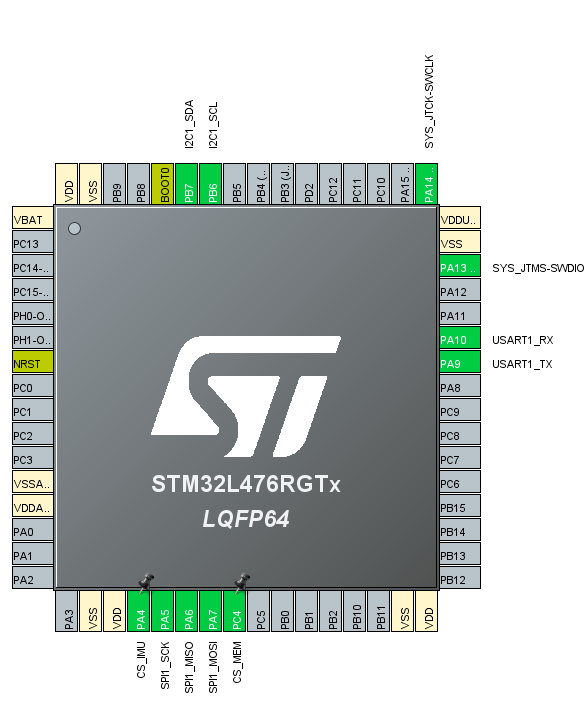
\includegraphics[width=0.62\textwidth]{figuras/stm32.png}
    \caption{Asignación de pines del STM32L476RGT6 realizada en STM32CubeMX\@.}%
    \label{fig:stm32_pinout}
\end{figure}
\subsection{Microcontrolador seleccionado}
Se selecciona el STM32L476RGT6 porque permite utilizar
simultáneamente las interfaces previstas y ofrece el mayor margen
de memoria Flash y RAM de los candidatos estudiados. Dispone
también de FPU, que puede resultar útil al ampliar el
procesamiento de las medidas. Frente al STM32F401RET6, presenta
una menor corriente en las condiciones de referencia consultadas,
con frecuencias máximas próximas.

\begin{table}[H]
\centering
\small
\renewcommand{\arraystretch}{1.25}
\begin{tabularx}{\textwidth}{
    >{\raggedright\arraybackslash}X
    >{\centering\arraybackslash}p{3.5cm}
    >{\centering\arraybackslash}p{3.5cm}
    >{\centering\arraybackslash}p{3.5cm}
}
\toprule
Criterio
& \shortstack{STM32G071\\RBT6}
& \shortstack{STM32F401\\RET6}
& \shortstack{STM32L476\\RGT6} \\
\midrule
Núcleo & Cortex-M0+ & Cortex-M4 & Cortex-M4 \\
Frecuencia máxima & 64 MHz & 84 MHz & 80 MHz \\
FPU & No & Sí & Sí \\
Flash & 128 KB & 512 KB & 1024 KB \\
RAM total & 36 KB & 96 KB & 128 KB \\
Interfaces y pines previstos & Compatibles & Compatibles & Compatibles \\
Corriente de referencia en Run
& 6,4 mA & 12,5 mA & 10,2 mA \\
Energía de referencia en 120 s
& 2,53 J & 4,95 J & 4,04 J \\
Tiempo de procesamiento de la aplicación
& No medido & No medido & No medido \\
\bottomrule
\end{tabularx}
\caption{Resumen de los candidatos. La energía se ha calculado
suponiendo \(3{,}3\,\mathrm{V}\) y \(120\,\mathrm{s}\) continuos en modo
\textit{Run}. Las corrientes proceden de ensayos de referencia con
condiciones y código diferentes; los valores de energía no predicen
el consumo real durante el vuelo.}%
\label{tab:comparacion_final_uc}
\end{table}

El STM32G071RBT6 no queda descartado por falta demostrada de
memoria o de capacidad de cálculo. Su corriente de referencia es
menor, pero dispone de menos memoria y carece de FPU\@. No se ha
medido aún el tiempo de ejecución ni el consumo de la aplicación
en ninguno de los candidatos; por tanto, la selección prioriza
el margen para desarrollar la aviónica prevista y no presupone
un menor consumo real durante el vuelo.

% ================================================================

% La elección final se realizará después de comparar:
% - periféricos disponibles;
% - compatibilidad de pines;
% - consumo;
% - DMA;
% - memoria;
% - capacidad de cálculo;
% - margen de expansión.

\newpage
% ================================================================
\section{Configuración básica en STM32CubeMX}
% ================================================================

La configuración parte de la arquitectura propuesta en el
apartado anterior y de la asignación de pines recogida en la
Tabla~\ref{tab:asignacion_pines}. Se utiliza I\textsuperscript{2}C1
para comunicar el microcontrolador con un barómetro, del que se
obtendrá la presión empleada para estimar la altura. SPI1 se
reserva para la IMU y una memoria externa donde registrar los
datos de vuelo. Por último, USART1 permitirá recibir los datos
de un receptor GNSS mediante comunicación serie asíncrona.

La IMU y la memoria externa compartirán las líneas SCK, MOSI y
MISO de SPI1. Cada dispositivo tendrá una señal de selección
independiente, controlada mediante un GPIO\@: \texttt{CS\_IMU}
en PA4 y \texttt{CS\_MEM} en PC4. Ambas señales permanecerán
inactivas a nivel alto; para iniciar una transferencia se pondrá
a nivel bajo únicamente la del dispositivo correspondiente y
se devolverá a nivel alto al terminar. Esta disposición permite
utilizar un solo periférico SPI para ambos dispositivos, siempre
que se respeten los parámetros de comunicación exigidos por
cada uno. Configuramos también la interfaz SWD para la programación y
depuración mediante ST-LINK\@.



% ================================================================
\subsection{Configuración del bus SPI}
% ================================================================

% Explicación de la configuración elegida.
% Se añadirán capturas de STM32CubeMX cuando corresponda.
Se configura SPI1 en modo maestro y dúplex completo. El
microcontrolador inicia las transferencias y genera la señal de reloj
SCK, mientras que las líneas MOSI y MISO permiten transmitir y recibir
bits durante los mismos ciclos de reloj. Esta configuración permite
atender las operaciones de lectura y escritura previstas para la IMU
y la memoria externa.

La señal NSS gestionada por hardware se deshabilita porque la IMU y
la memoria externa comparten SPI1, pero necesitan señales de selección
independientes. Para ello se asignan dos salidas GPIO a sus respectivos
CS\@. Suponiendo dispositivos con selección activa a nivel bajo, ambas
salidas permanecen inicialmente a nivel alto y el programa baja
únicamente el CS del dispositivo con el que realiza la transferencia.

Se seleccionan tramas de 8 bits para manejar las órdenes y los datos
como bytes en el programa. Las medidas que ocupen más de un byte se
recibirán mediante transferencias consecutivas, manteniendo activo el
CS correspondiente durante la operación. Esta elección se verificará
con los protocolos de la IMU y la memoria externa seleccionadas.

\begin{figure}[H]
    \centering

    \begin{minipage}[t]{0.44\textwidth}
        \centering
        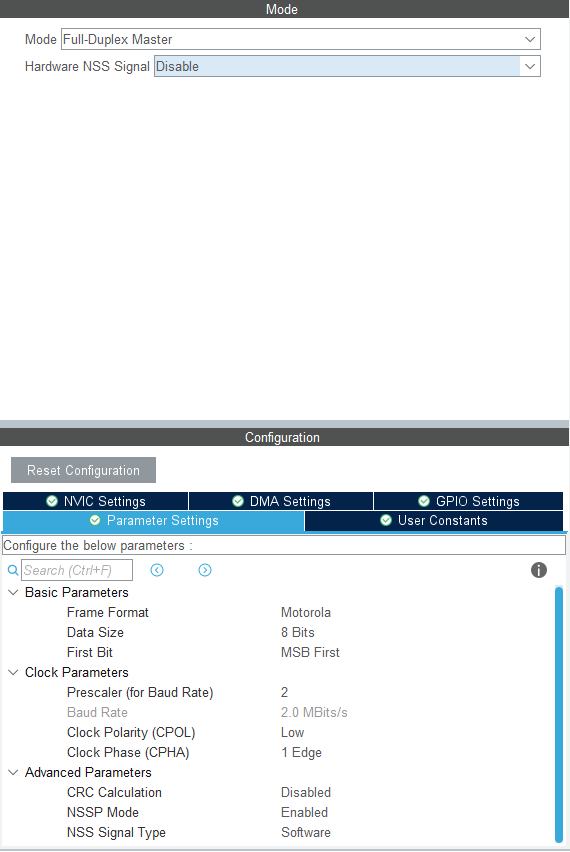
\includegraphics[
            width=\linewidth,
            trim=0 575bp 0 0,
            clip
        ]{figuras/spi_configuracion.png}
    \end{minipage}
    \hfill
    \begin{minipage}[t]{0.54\textwidth}
        \centering
        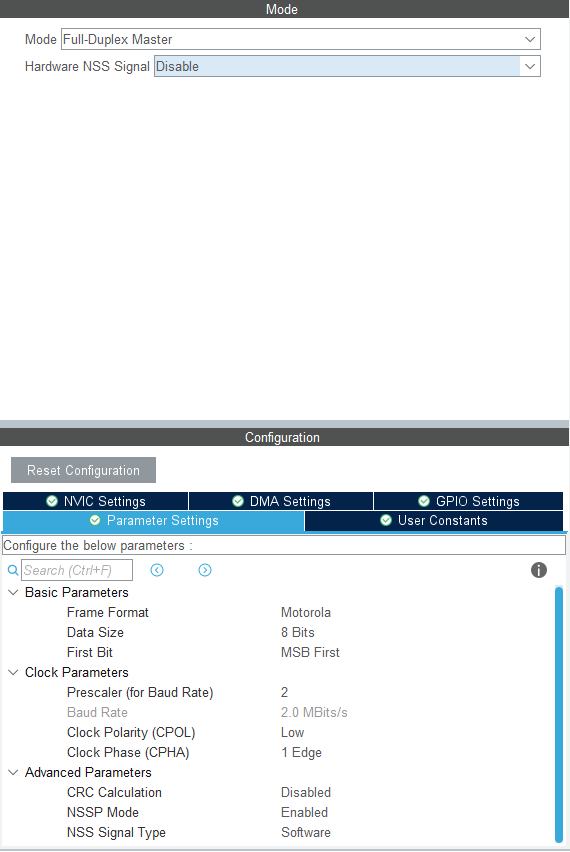
\includegraphics[
            width=\linewidth,
            trim=0 0 0 315bp,
            clip
        ]{figuras/spi_configuracion.png}
    \end{minipage}

    \caption{Configuración de SPI1 en STM32CubeMX\@: modo de funcionamiento
    y parámetros de transferencia.}%
    \label{fig:configuracion_spi1}
\end{figure}

% ================================================================
\subsection{Configuración del bus I\texorpdfstring{$^2$}{2}C}
% ================================================================

% Explicación de la configuración elegida.
Se configura I2C1 a 100 kHz para comunicar el microcontrolador con
el barómetro. Como estimación inicial, una lectura de tres bytes de
presión, junto con los bytes necesarios para direccionar el dispositivo
y el registro, ocuparía aproximadamente 0,54 ms de transmisión. Este
tiempo es inferior a los 10 ms entre muestras previstos para una tasa
de 100 Hz. Antes de fijar dicha tasa se comprobarán el protocolo y
el tiempo de conversión del barómetro seleccionado.

Se emplea direccionamiento I2C de 7 bits. Vamos a trabajar con un único uC, por lo que no necesita una dirección propia en esta
configuración. La dirección del barómetro se establecerá al seleccionar
el componente concreto.

\begin{figure}[H]
    \centering

    \begin{minipage}[t]{0.44\textwidth}
        \centering
        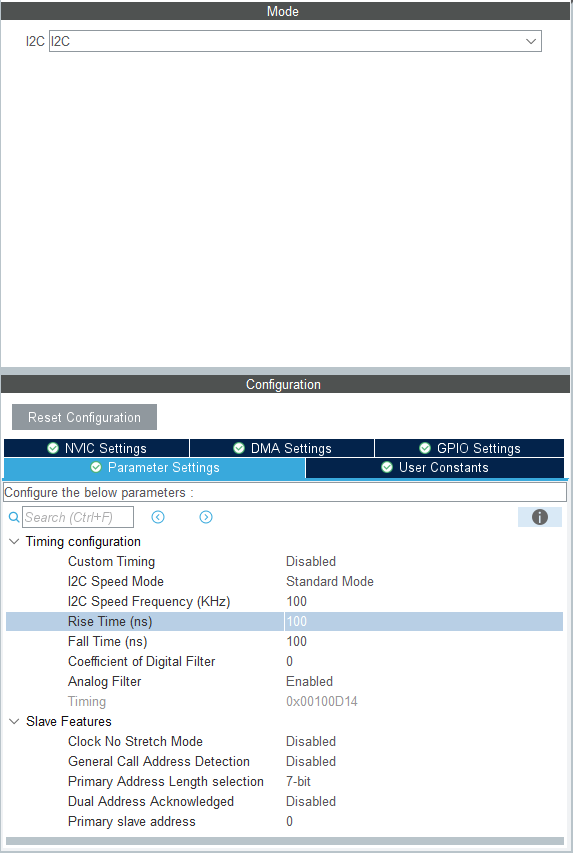
\includegraphics[
            width=\linewidth,
            trim=0 575bp 0 0,
            clip
        ]{figuras/i2c_configuracion.png}
    \end{minipage}
    \hfill
    \begin{minipage}[t]{0.54\textwidth}
        \centering
        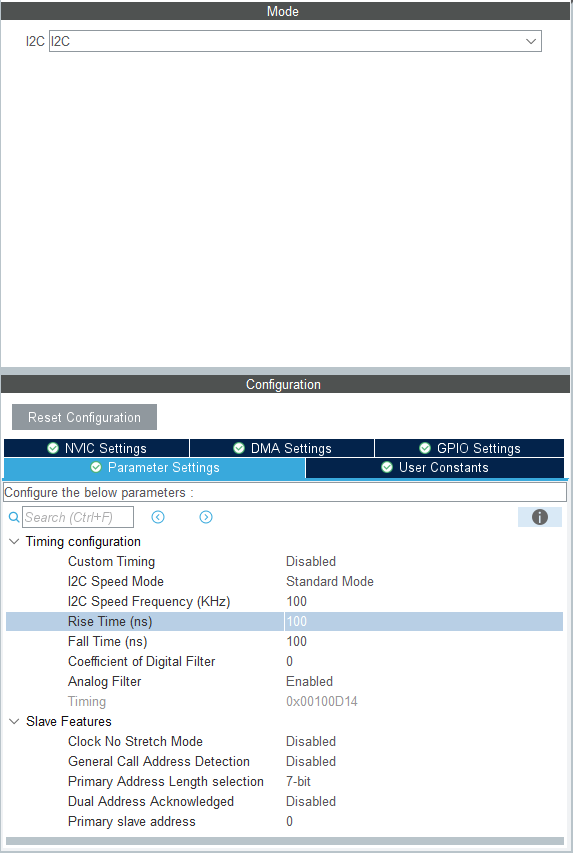
\includegraphics[
            width=\linewidth,
            trim=0 0 0 315bp,
            clip
        ]{figuras/i2c_configuracion.png}
    \end{minipage}

    \caption{Configuración de I2C1 en STM32CubeMX\@: modo de funcionamiento
    y parámetros de transferencia.}%
    \label{fig:configuracion_i2c1}
\end{figure}
% ================================================================
\subsection{Configuración de ST-LINK}
% ================================================================

% Explicación de la interfaz SWD y de su configuración.
Para permitir la programación y depuración con ST-LINK se selecciona
\textit{Serial Wire} en System Core/SYS de STM32CubeMX\@. Esta
configuración reserva PA13 para SWDIO y PA14 para SWCLK\@. En una placa
física, el conector de depuración incluirá también una masa común y
la tensión de referencia del circuito, necesaria para que el
programador utilice niveles eléctricos compatibles. Se prevé además
la conexión NRST, que facilita reiniciar el microcontrolador y
recuperar el acceso de depuración si el programa cargado dificulta
la conexión.

% Breve resumen de la elección del microcontrolador y de la
% configuración realizada.
\newpage
\renewcommand{\refname}{Referencias}

\begin{thebibliography}{9}
\raggedright{}

\bibitem{st_l476}
STMicroelectronics. (2024).
\textit{STM32L476xx: Ultra-low-power Arm Cortex-M4 32-bit MCU+FPU}
(DS10198, rev. 11).
\url{https://www.st.com/resource/en/datasheet/stm32l476rg.pdf}

\bibitem{st_g071}
STMicroelectronics. (2025).
\textit{STM32G071x\mbox{8} y STM32G071xB\@: Arm Cortex-M0+ 32-bit MCU}
(DS12232, rev. 5).
\url{https://www.st.com/resource/en/datasheet/stm32g071rb.pdf}

\bibitem{st_cubemx}
STMicroelectronics. (2026a).
\textit{STM32CubeMX for STM32 configuration and initialization
C code generation} (UM1718).
\url{https://www.st.com/resource/en/user_manual/dm00104712-stm32cubemx-for-stm32-configuration-and-initialization-c-code-generation-stmicroelectronics.pdf}

\bibitem{st_f401}
STMicroelectronics. (2026b).
\textit{STM32F401xD/STM32F401xE\@: Arm Cortex-M4 32-bit MCU+FPU}
(DS10086, rev. 5).
\url{https://www.st.com/resource/en/datasheet/stm32f401re.pdf}

\bibitem{farnell}
Farnell.\ (sin fecha).
\textit{Microcontroladores ARM\@: catálogo y precios}.
Recuperado el 24 de septiembre de 2026, de
\url{https://es.farnell.com/c/semiconductores-circuitos-integrados/microcontroladores/microcontroladores-arm}

\end{thebibliography}
\newpage
\appendix

\section{Código empleado en la estimación de memoria}%
\label{anexo:estimacion_flash}

Los siguientes fragmentos corresponden a las funciones incorporadas
progresivamente al proyecto generado por STM32CubeMX\@. Las entradas
ficticias permiten que las funciones se ejecuten en el programa compilado;
no representan medidas obtenidas de un sensor.

\subsection{Filtro de altura}

\begin{lstlisting}[caption={Filtro exponencial utilizado en la prueba.},
label={lst:filtro_altura}]
static float FiltrarAltura(float altura_nueva, float altura_anterior)
{
  const float alpha = 0.25f;  /* Valor de prueba */
  return altura_anterior + alpha * (altura_nueva - altura_anterior);
}
\end{lstlisting}

\subsection{Conversión de presión en altura relativa}

La función siguiente utiliza \texttt{logf}, por lo que se añadió
\texttt{\#include <math.h>} al archivo \texttt{main.c}.

\begin{lstlisting}[caption={Conversión aproximada de presión a altura relativa.},
label={lst:presion_altura}]
static float AlturaDesdePresion(float presion_pa,
                               float presion_inicial_pa)
{
  const float R = 287.05f;     /* J/(kg K), aire seco */
  const float T = 288.15f;     /* K, valor supuesto */
  const float g = 9.80665f;    /* m/s2 */

  return (R * T / g) * logf(presion_inicial_pa / presion_pa);
}
\end{lstlisting}

\subsection{Ejecución con entradas ficticias}

\begin{lstlisting}[caption={Generación de presión ficticia, conversión
y filtrado de altura.},label={lst:prueba_altura}]
static uint32_t instante_anterior = 0U;
static uint8_t primera_medida = 1U;
static float altura_filtrada = 0.0f;
static volatile float resultado_prueba = 0.0f;

uint32_t instante_actual = HAL_GetTick();

if ((uint32_t)(instante_actual - instante_anterior) >= 10U)
{
  instante_anterior = instante_actual;

  float presion_prueba_pa =
      101325.0f - 10.0f * (float)((instante_actual / 10U) % 100U);
  float altura_nueva =
      AlturaDesdePresion(presion_prueba_pa, 101325.0f);

  if (primera_medida)
  {
    altura_filtrada = altura_nueva;
    primera_medida = 0U;
  }
  else
  {
    altura_filtrada = FiltrarAltura(altura_nueva,
                                   altura_filtrada);
  }

  resultado_prueba = altura_filtrada;
}
\end{lstlisting}
\section{Simulación de presión y detección de descenso}%
\label{anexo:simulacion_descenso}

La versión ampliada del programa sustituye la presión ficticia
empleada inicialmente por una señal de 120 segundos. La presión
disminuye desde 101\,325 Pa hasta 34\,900 Pa durante los primeros
60 segundos y después vuelve al valor inicial linealmente. Con el modelo
barométrico simplificado utilizado, la presión mínima corresponde
a una altura próxima a 9 km.

\subsection{Simulación de la presión}

El programa comprueba si han transcurrido al menos 10 ms desde la
muestra anterior. Este intervalo establece una frecuencia
de procesamiento de 100 Hz.

\begin{lstlisting}[
    caption={Generación de una presión simulada con ascenso y descenso.},
    label={lst:simulacion_presion}
]
uint32_t instante_actual = HAL_GetTick();

if ((uint32_t)(instante_actual - instante_anterior) >= 10U)
{
    instante_anterior = instante_actual;

    float tiempo_s =
        (float)(instante_actual % 120000U) / 1000.0f;
    const float presion_inicio_pa = 101325.0f;
    const float presion_minima_pa = 34900.0f;
    float presion_prueba_pa;

    if (tiempo_s <= 60.0f)
    {
        presion_prueba_pa = presion_inicio_pa
            + (presion_minima_pa - presion_inicio_pa)
              * tiempo_s / 60.0f;
    }
    else
    {
        presion_prueba_pa = presion_minima_pa
            + (presion_inicio_pa - presion_minima_pa)
              * (tiempo_s - 60.0f) / 60.0f;
    }

    float altura_nueva =
        AlturaDesdePresion(presion_prueba_pa,
                           presion_inicio_pa);

    /* A continuacion se filtra y analiza altura_nueva. */
}
\end{lstlisting}

\subsection{Historial de alturas}

La altura calculada se filtra mediante la función del
Listado~\ref{lst:filtro_altura}. Se conserva la máxima altura
filtrada y se utiliza un historial circular de 20 medidas para
comparar la altura actual con la obtenida aproximadamente
0,2 segundos antes.

\begin{lstlisting}[
    caption={Almacenamiento de alturas y cálculo de su variación.},
    label={lst:historial_alturas}
]
static float historial_alturas[20] = {0};
static uint8_t indice_historial = 0U;
static uint8_t muestras_guardadas = 0U;
static float altura_maxima = 0.0f;
static volatile float cambio_altura_02s = 0.0f;

/* Tras calcular altura_filtrada: */
if (altura_filtrada > altura_maxima)
{
    altura_maxima = altura_filtrada;
}

if (muestras_guardadas == 20U)
{
    cambio_altura_02s =
        altura_filtrada
        - historial_alturas[indice_historial];

    /* Aqui se evalua la deteccion de descenso. */
}
else
{
    muestras_guardadas++;
}

historial_alturas[indice_historial] = altura_filtrada;
indice_historial =
    (uint8_t)((indice_historial + 1U) % 20U);
\end{lstlisting}

\subsection{Indicador lógico de descenso}

La detección combina una caída respecto a la máxima altura
registrada con una variación negativa en la ventana de
0,2 segundos. Se requieren 50 comprobaciones favorables,
tolerando hasta dos resultados desfavorables consecutivos.
Una vez confirmado el descenso, el indicador permanece activo.

\begin{lstlisting}[
    caption={Condición de prueba para confirmar el descenso.},
    label={lst:deteccion_descenso}
]
static uint8_t confirmaciones_descenso = 0U;
static uint8_t fallos_consecutivos = 0U;
static volatile uint8_t descenso_detectado = 0U;

/* Dentro del bloque con 20 alturas ya almacenadas: */
if (descenso_detectado == 0U)
{
    const float caida_minima_desde_maximo_m = 2.0f;
    const float descenso_minimo_02s_m = 1.0f;

    if ((altura_maxima - altura_filtrada >=
         caida_minima_desde_maximo_m) &&
        (cambio_altura_02s <=
         -descenso_minimo_02s_m))
    {
        fallos_consecutivos = 0U;
        confirmaciones_descenso++;

        if (confirmaciones_descenso >= 50U)
        {
            descenso_detectado = 1U;
        }
    }
    else
    {
        fallos_consecutivos++;

        if (fallos_consecutivos >= 3U)
        {
            confirmaciones_descenso = 0U;
            fallos_consecutivos = 0U;
        }
    }
}
\end{lstlisting}

Los umbrales de 2 m, 1 m y 50 comprobaciones se han utilizado
para construir el prototipo y estimar su ocupación de memoria.
La compilación no demuestra que la detección funcione ante
medidas reales o que sea adecuada para activar un mecanismo
de vuelo. El código implementa un indicador de descenso, no
una máquina de estados completa.
En el ejercicio 2 se conserva este esquema de cálculo de altura y detección
de descenso, pero se sustituye la presión simulada por las muestras nuevas
obtenidas de dos barómetros LPS22DF. También se añaden la configuración y
lectura parcial de la IMU y la recepción de bytes del GNSS. La integración
de esos componentes y sus límites se describen en el informe del ejercicio 2.
\end{document}
